\documentclass{article}
\usepackage{textcomp}
\usepackage[utf8x]{inputenc}
\usepackage{graphicx}
\usepackage{xcolor}
\usepackage[most]{tcolorbox}
\usepackage{todonotes}
\usepackage{float}
\usepackage[center]{titlesec}

\begin{document}

  \begin{titlepage}

    \newcommand{\HRule}{\rule{\linewidth}{0.5mm}} % Defines a new command for the horizontal lines, change thickness here

    \center % Center everything on the page

%----------------------------------------------------------------------------------------
%	HEADING SECTIONS
%----------------------------------------------------------------------------------------

    \textsc{\LARGE Technical University of Moldova}\\[1.5cm]
    \textsc{\Large Special Mathematics}\\[0.5cm] % Major heading such as course name

%----------------------------------------------------------------------------------------
%	TITLE SECTION
%----------------------------------------------------------------------------------------

    \HRule \\[0.4cm]
    { \huge \bfseries Laboratory No.4}\\[0.4cm] % Title of your document
    \HRule \\[1.5cm]

%----------------------------------------------------------------------------------------
%	AUTHOR SECTION
%----------------------------------------------------------------------------------------

    \begin{minipage}{0.4\textwidth}
      \begin{flushleft} \large
        \emph{Author:}\\
          st. Polina \textsc{Gore}\\ gr. FAF-161 % Your name
      \end{flushleft}
    \end{minipage}
~
    \begin{minipage}{0.4\textwidth}
      \begin{flushright} \large
        \emph{Supervisor:} \\
        Victor \textsc{Țurcanu} % Supervisor's Name
      \end{flushright}
    \end{minipage}\\[2cm]

%----------------------------------------------------------------------------------------
%	DATE SECTION
%----------------------------------------------------------------------------------------

    {\large \today}\\[2cm] % Date, change the \today to a set date if you want to be precise

%----------------------------------------------------------------------------------------
%	LOGO SECTION
%----------------------------------------------------------------------------------------
    
\includegraphics[width=7cm]{utm2.png}\\[1cm] % Include a department/university logo - this will require the graphicx package

%----------------------------------------------------------------------------------------

    \vfill % Fill the rest of the page with whitespace

  \end{titlepage}

%----------------------------------------------------------------------------------------
%----------------------------------------------------------------------------------------

  \newpage
  \pagenumbering{arabic}

  % -------------- PROBLEM 1------------------------------------------------------

  \section{Understanding logical operations}
    Here you have \textit{image} \underline{1} that can be obtained by running
    the code from \textit{listing} \underline{1}.\\
    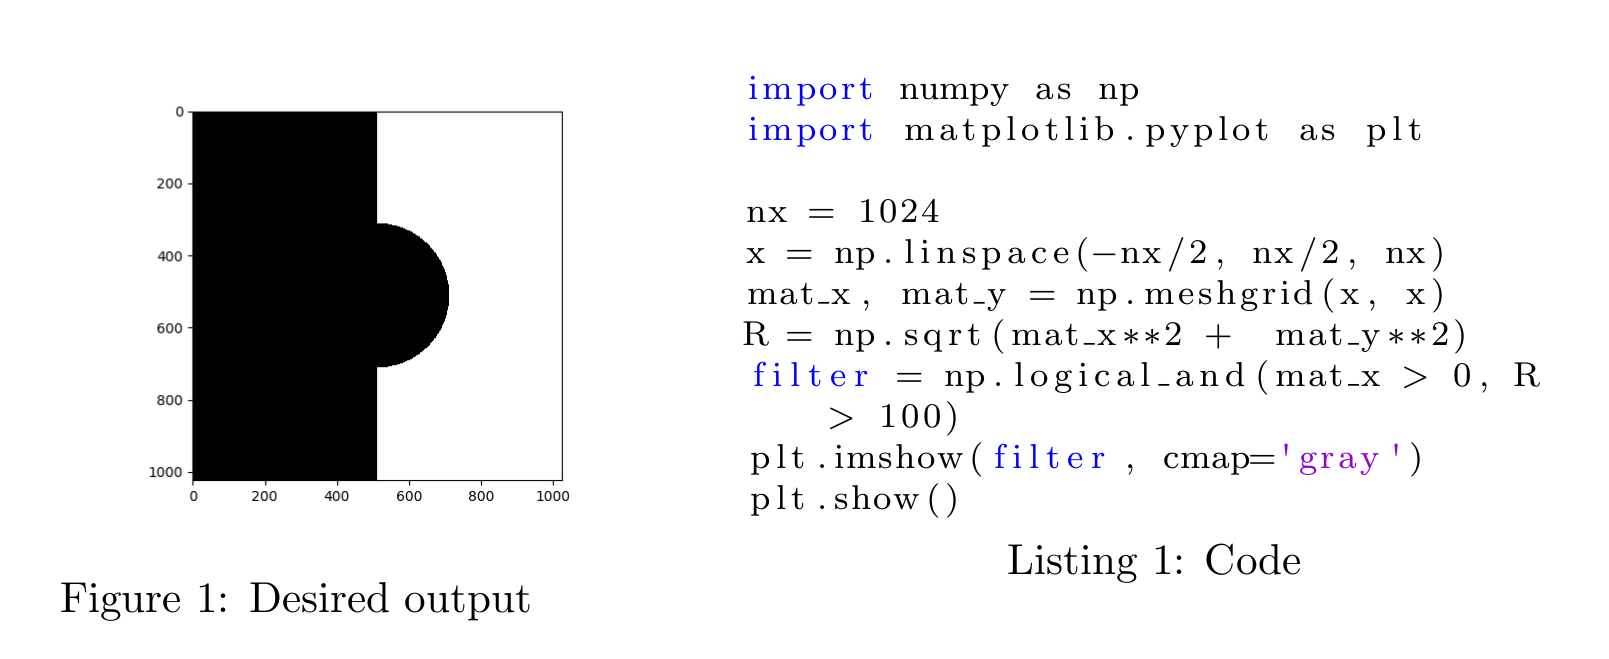
\includegraphics[width=13cm]{ex1.png}
    Change it to obtain the following images.\\

  \vspace{2em}

  \subsection{Solution}
    \emph{1)} Either \(x < 0\) or \(R > 100\) \hfill
    \emph{2)} (\(R > 100\) or \(y > 0)\) and (\(R < 100\) or \(x > 0)\)\\
    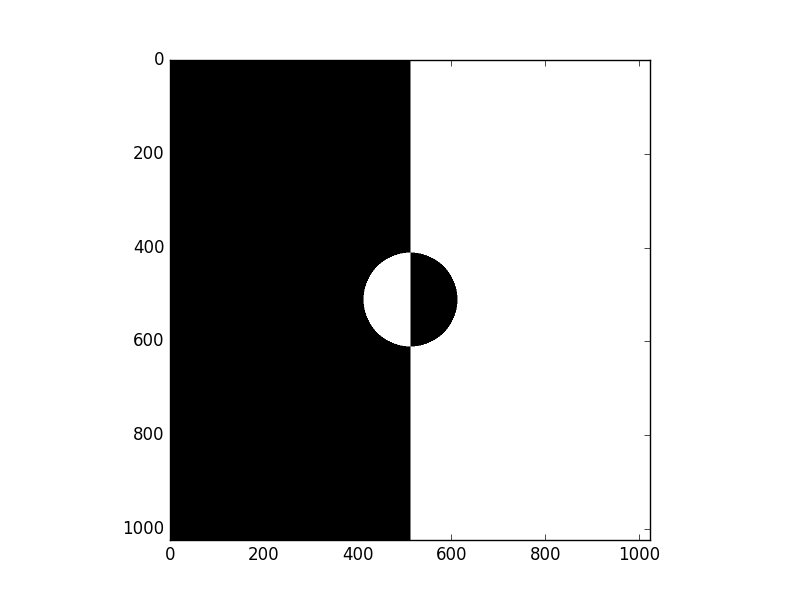
\includegraphics[width=8cm]{figure_1.png}
    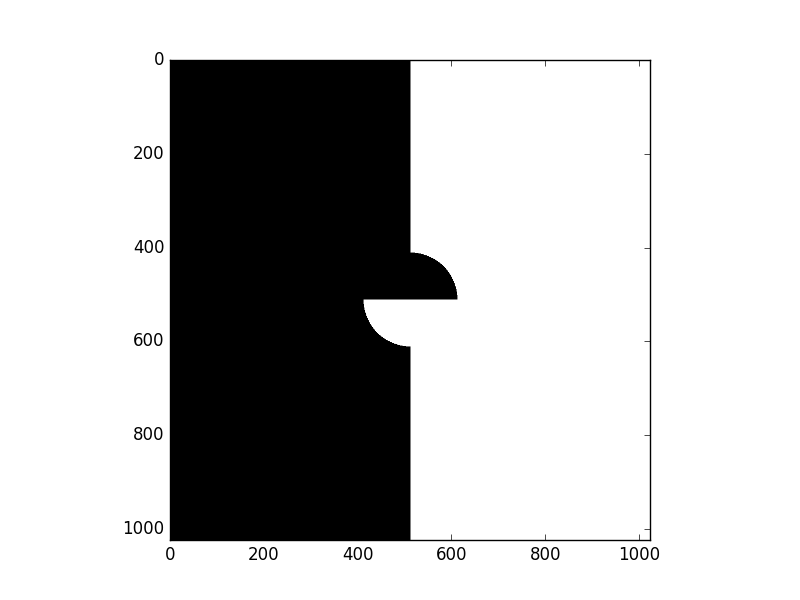
\includegraphics[width=8cm]{figure_2.png}\\
    \newpage
    \emph{3)} Neither \(y < 0\) nor \(x < 0\) \hfill
    \emph{4)} \(R < 512\) or (either \(y < 0\) or \(x > 0)\)\\
    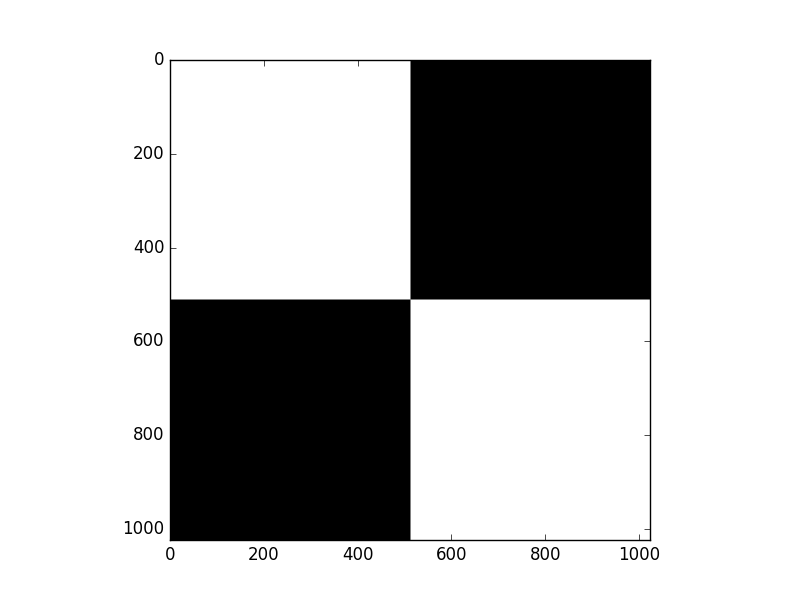
\includegraphics[width=8cm]{figure_3.png}
    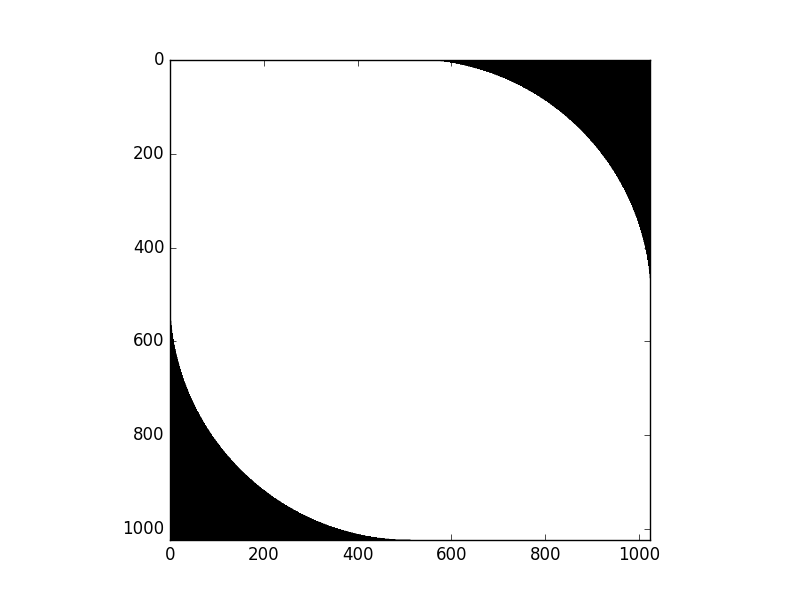
\includegraphics[width=8cm]{figure_4.png}\\
    \emph{5)} Either \(y > 0\) or \(R > 512\) \hfill
    \emph{6)} \(x > 0\) and \(R > 512\)\\
    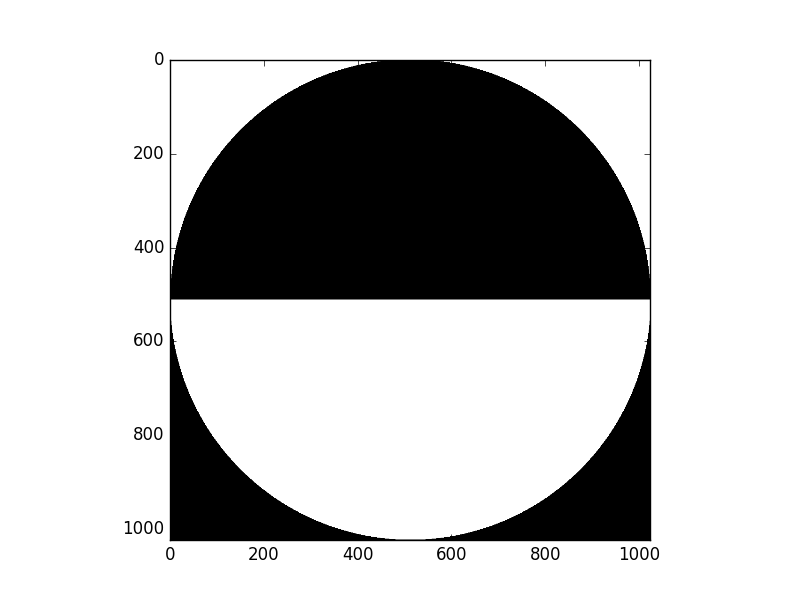
\includegraphics[width=8cm]{figure_5.png}
    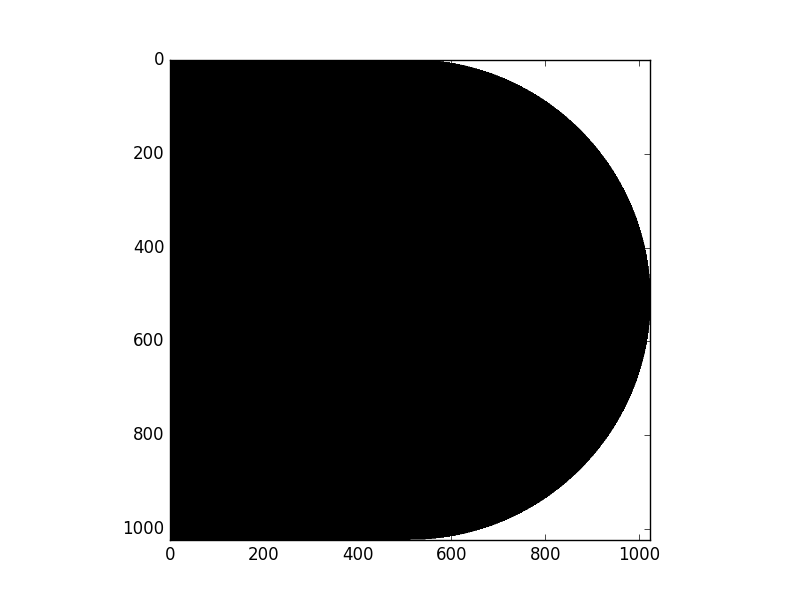
\includegraphics[width=8cm]{figure_6.png}\\


  \newpage

  %----------------------PROBLEM 2----------------------------------------------

  \section{Leibniz harmonic triangle}
    Write a program that prints the harmonic triangle for the depth \emph{n},
    where \emph{n} is an input value.

  \vspace{3em}

  \subsection{Solution}
    \textit{\textbf{The Leibniz harmonic triangle} is a triangular arrangement of unit
    fractions in which the outermost diagonals consist of the reciprocals of the
    row numbers and each inner cell is the absolute value of the cell above
    minus the cell to the left.}\hfill (Wikipedia)\\

    This is the rule I used to \emph{'create'} the Leibniz triangle.

    \vspace{2em}
    \centerline{\emph{Examples:}}
    \vspace{2em}

    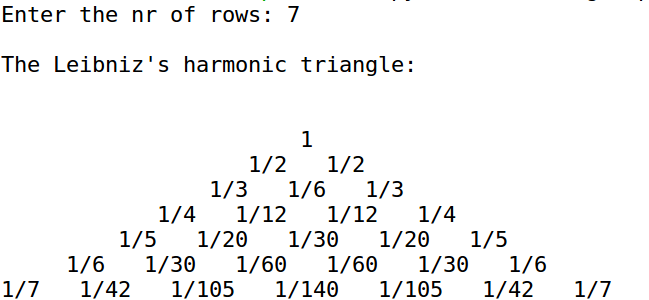
\includegraphics[width=8cm]{ex2b.png}\\

    \vspace{2em}
    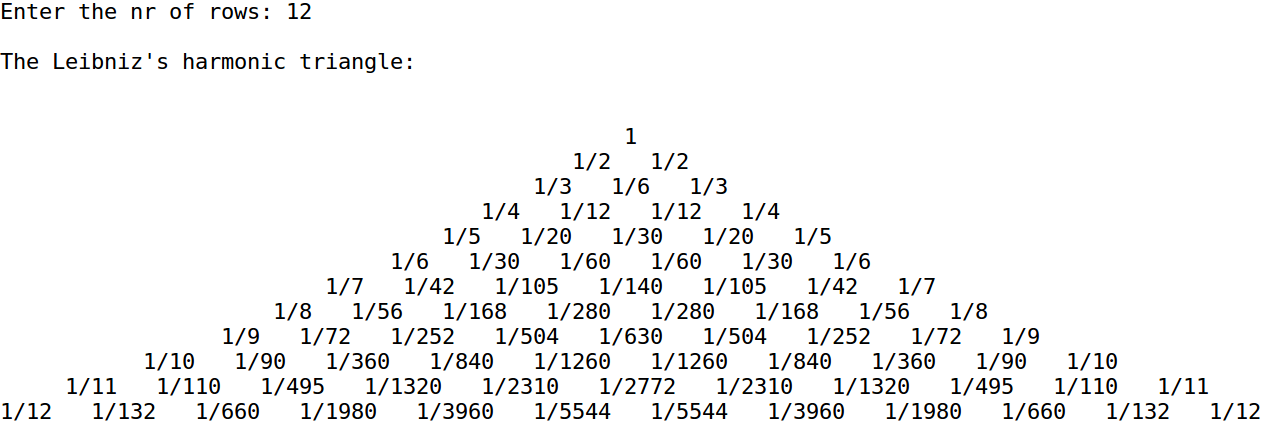
\includegraphics[width=15cm]{ex2c.png}


  \newpage

    %----------------------PROBLEM 3--------------------------------------------

    \section{Truth table solver}
      You have to write a program that computes the truth table for various
      expressions.\\
      The set of expressions are limited to:\\

      • \emph{and} operation

      • \emph{or} operation

      • \emph{not} operation

      • supports paranthesis

    \vspace{3em}

    \subsection{Solution}
      First of all, I checked the expression to be sure it's a working one
      using regular expressions (which needs the \emph{re} module).\\
      If it's not, exit with an error message, otherwise, evaluate it.\\
      To evaluate the expression, I used the \emph{eval} function, but before,
      I changed every sign (!, *, +) to the corresponding logical terms (not, and, or).\\
      And to make the truth table, I used the \emph{product} function from
      \emph{itertools} module which is the cross product of true and false repeated
      \emph{n} times (n = number of distinct variables).

      \vspace{3em}
      \centerline{\textbf{Examples:}}
      \vspace{2em}

      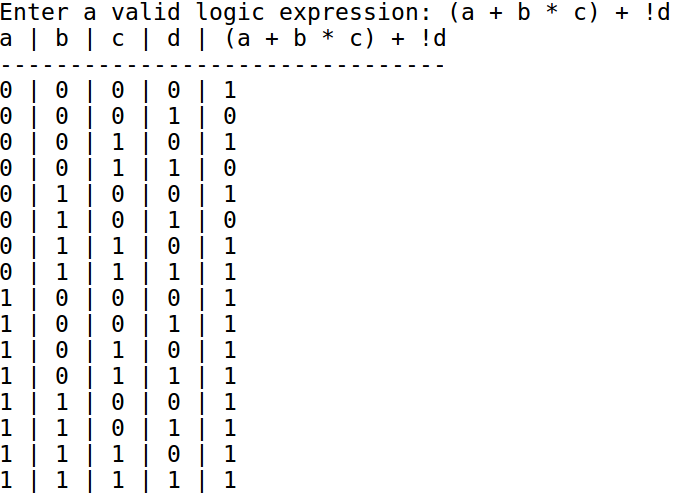
\includegraphics[width=7cm]{ex3a.png}\hfill
      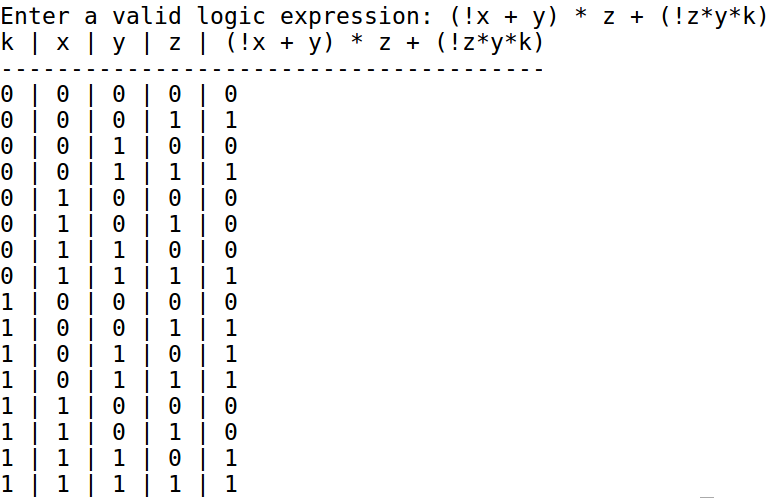
\includegraphics[width=8cm]{ex3b.png}

\end{document}
